\chapter{Additional Visual Results}
\label{app:visuals}

\Cref{fig:exp_qual_comparison,fig:exp_qual_cascade} in the main text (\Cref{sec:exp_qualitative}) show the cross-method comparison and the cascade stage internals for slice~17 under compound corruption. This appendix provides supplementary per-artifact qualitative comparisons on two additional test slices (3161 and~981) using the same figure format: a full reconstruction row and a magnified crop of the highest-artifact region, with PSNR~(dB) and SSIM annotated beneath each column. All figures show: Ground Truth~$|$ FBP~(noisy)~$|$ BM3D~$|$ RED-CNN~$|$ U-Net~(large)~$|$ Residual cascade~(dual-filter).

\section*{Slice 3161}

\begin{figure}[!htbp]
    \centering
    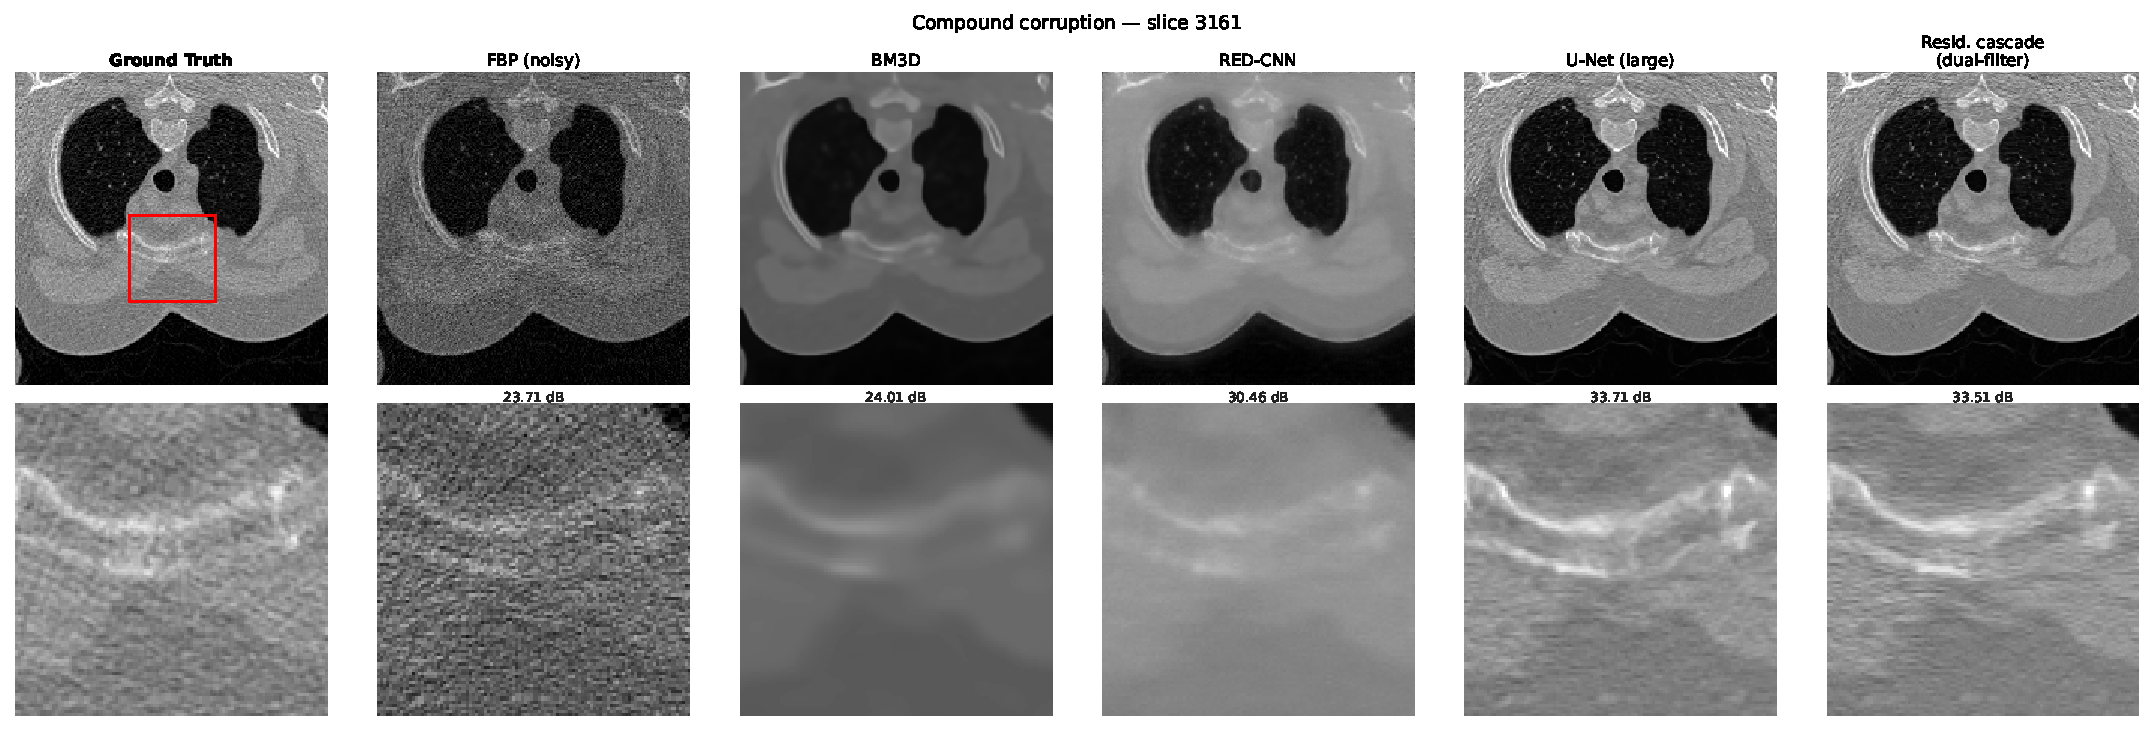
\includegraphics[width=\linewidth]{figures/results/fig_app_noise_only_slice3161.pdf}
    \caption[Slice~3161: noise-only condition.]{%
        Slice~3161, noise-only (low-dose Poisson noise, no physical artifacts).
        The learned models recover soft-tissue contrast suppressed by quantum noise;
        BM3D partially reduces noise but over-smooths fine structure.}
    \label{fig:app_qual_noise_3161}
\end{figure}

\begin{figure}[!htbp]
    \centering
    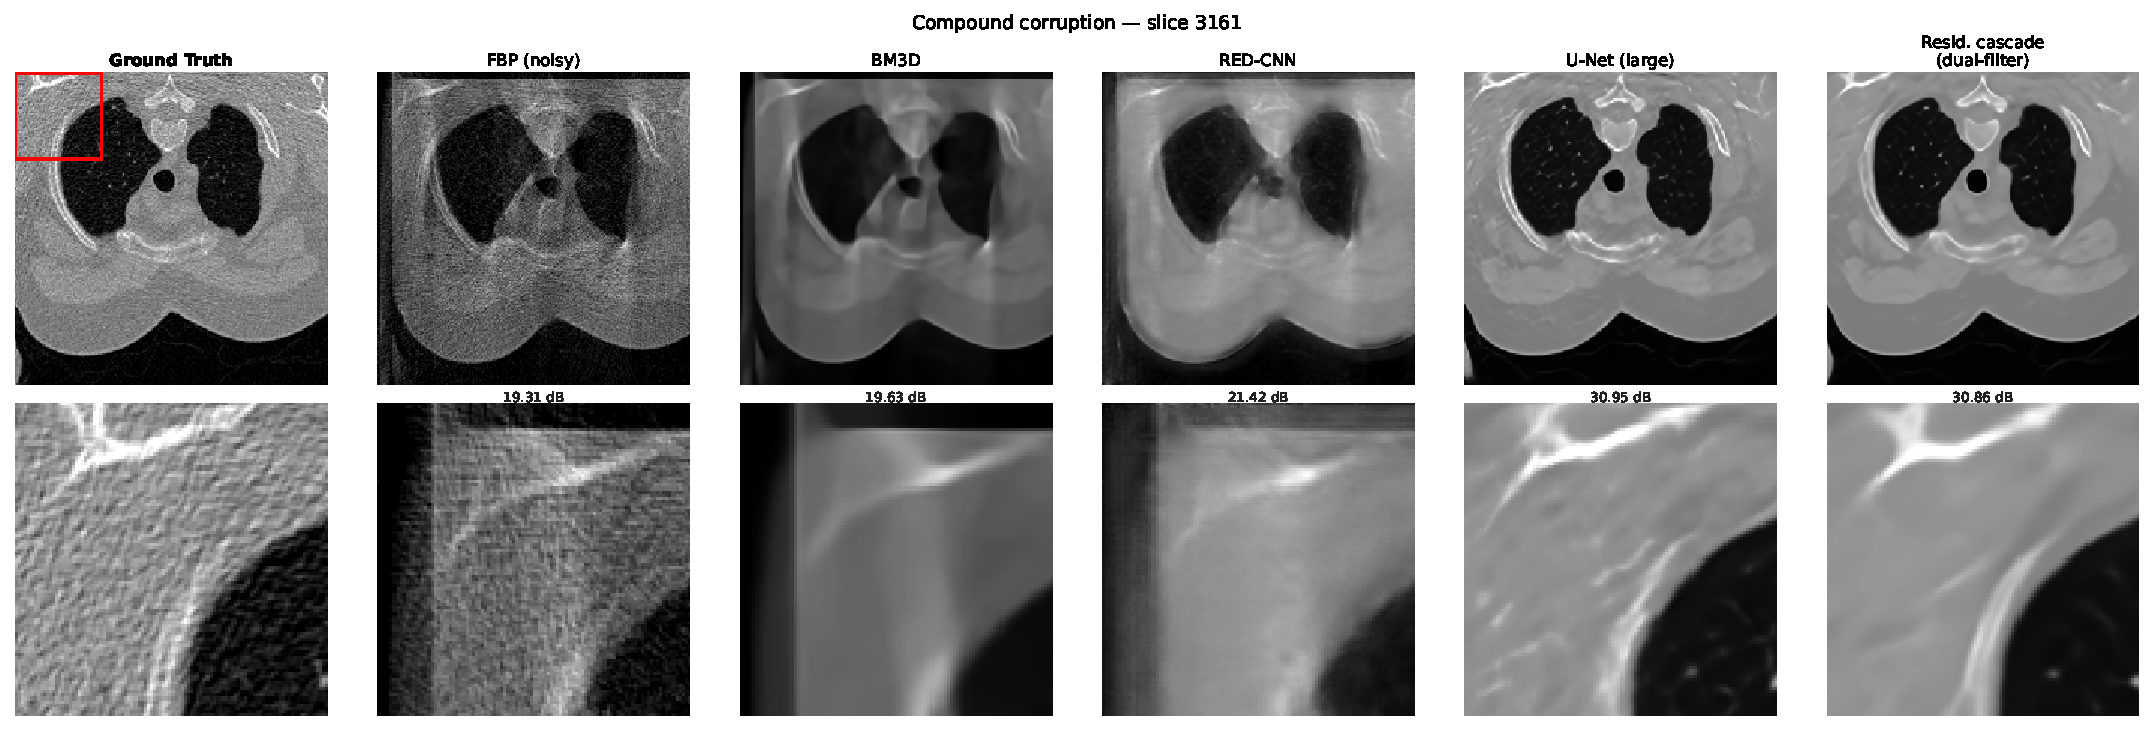
\includegraphics[width=\linewidth]{figures/results/fig_app_motion_slice3161.pdf}
    \caption[Slice~3161: motion artifact condition.]{%
        Slice~3161 with added respiratory motion artifacts (periodic sinogram shift,
        amplitude 10--20\,bins, 0.5--1.5 breathing cycles).
        Motion introduces edge blurring and ghosting visible in the zoomed crop;
        BM3D and RED-CNN partially mitigate noise but cannot resolve the motion
        inconsistency. Both U-Net variants substantially suppress the blurring.}
    \label{fig:app_qual_motion_3161}
\end{figure}

\begin{figure}[!htbp]
    \centering
    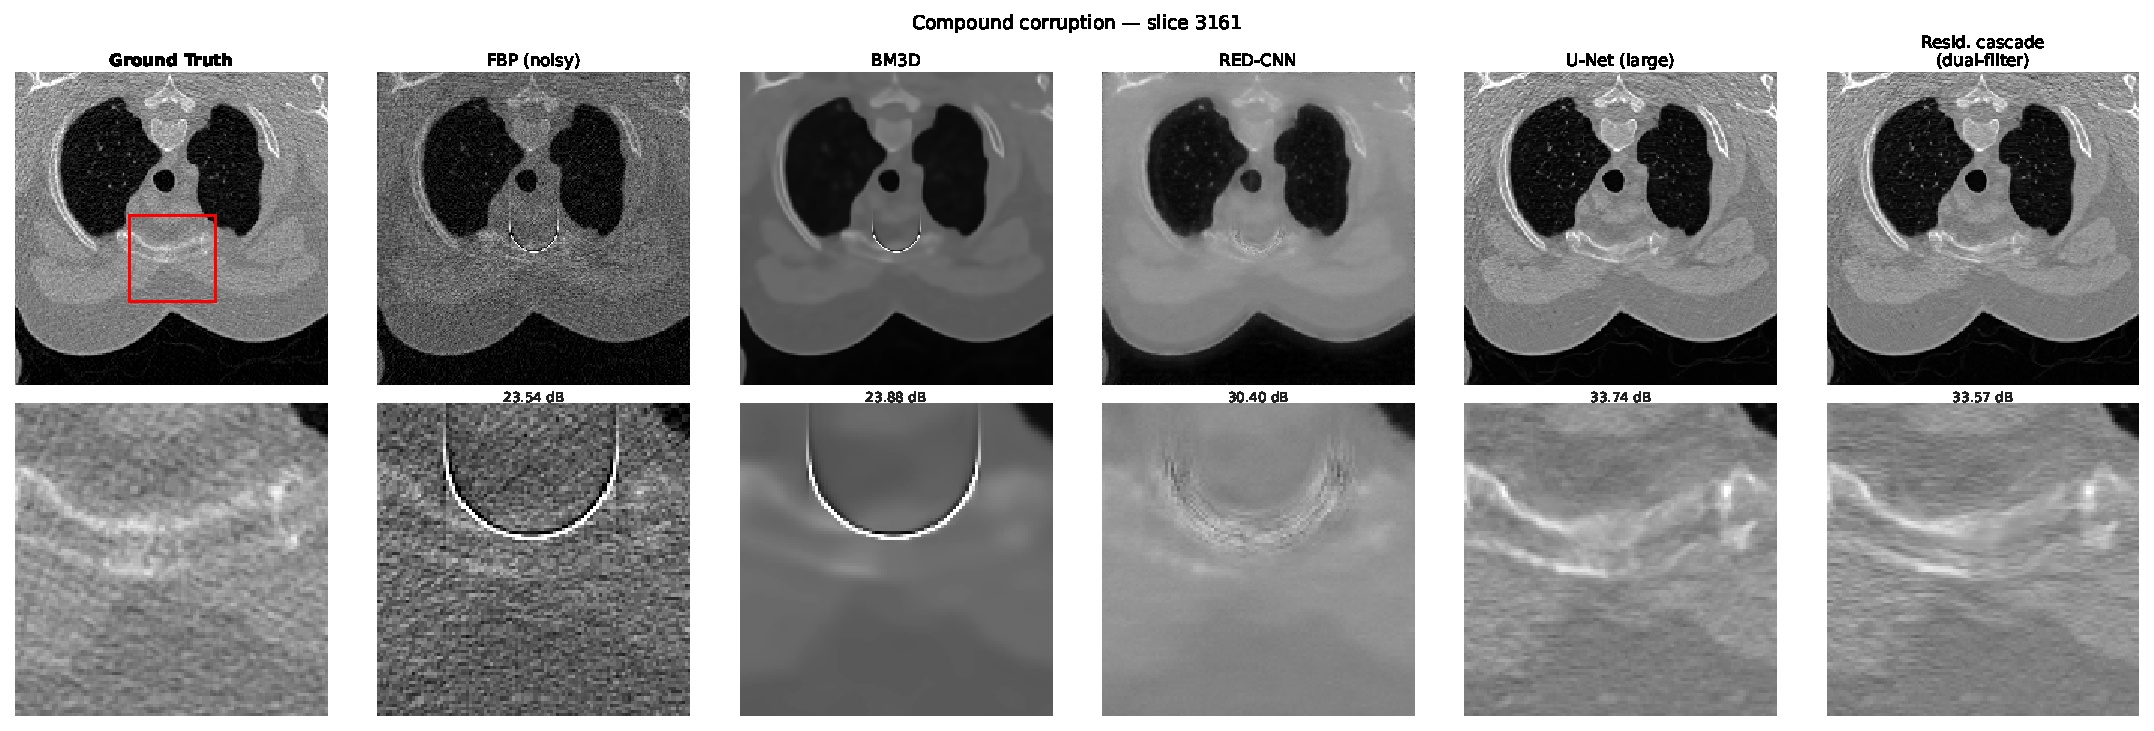
\includegraphics[width=\linewidth]{figures/results/fig_app_ring_slice3161.pdf}
    \caption[Slice~3161: ring artifact condition.]{%
        Slice~3161 with added detector ring artifacts (1--5 columns, gain error
        5--50\,\%). Concentric ring bands are visible in the FBP reconstruction;
        the learned models suppress these effectively while retaining tissue detail.}
    \label{fig:app_qual_ring_3161}
\end{figure}

\begin{figure}[!htbp]
    \centering
    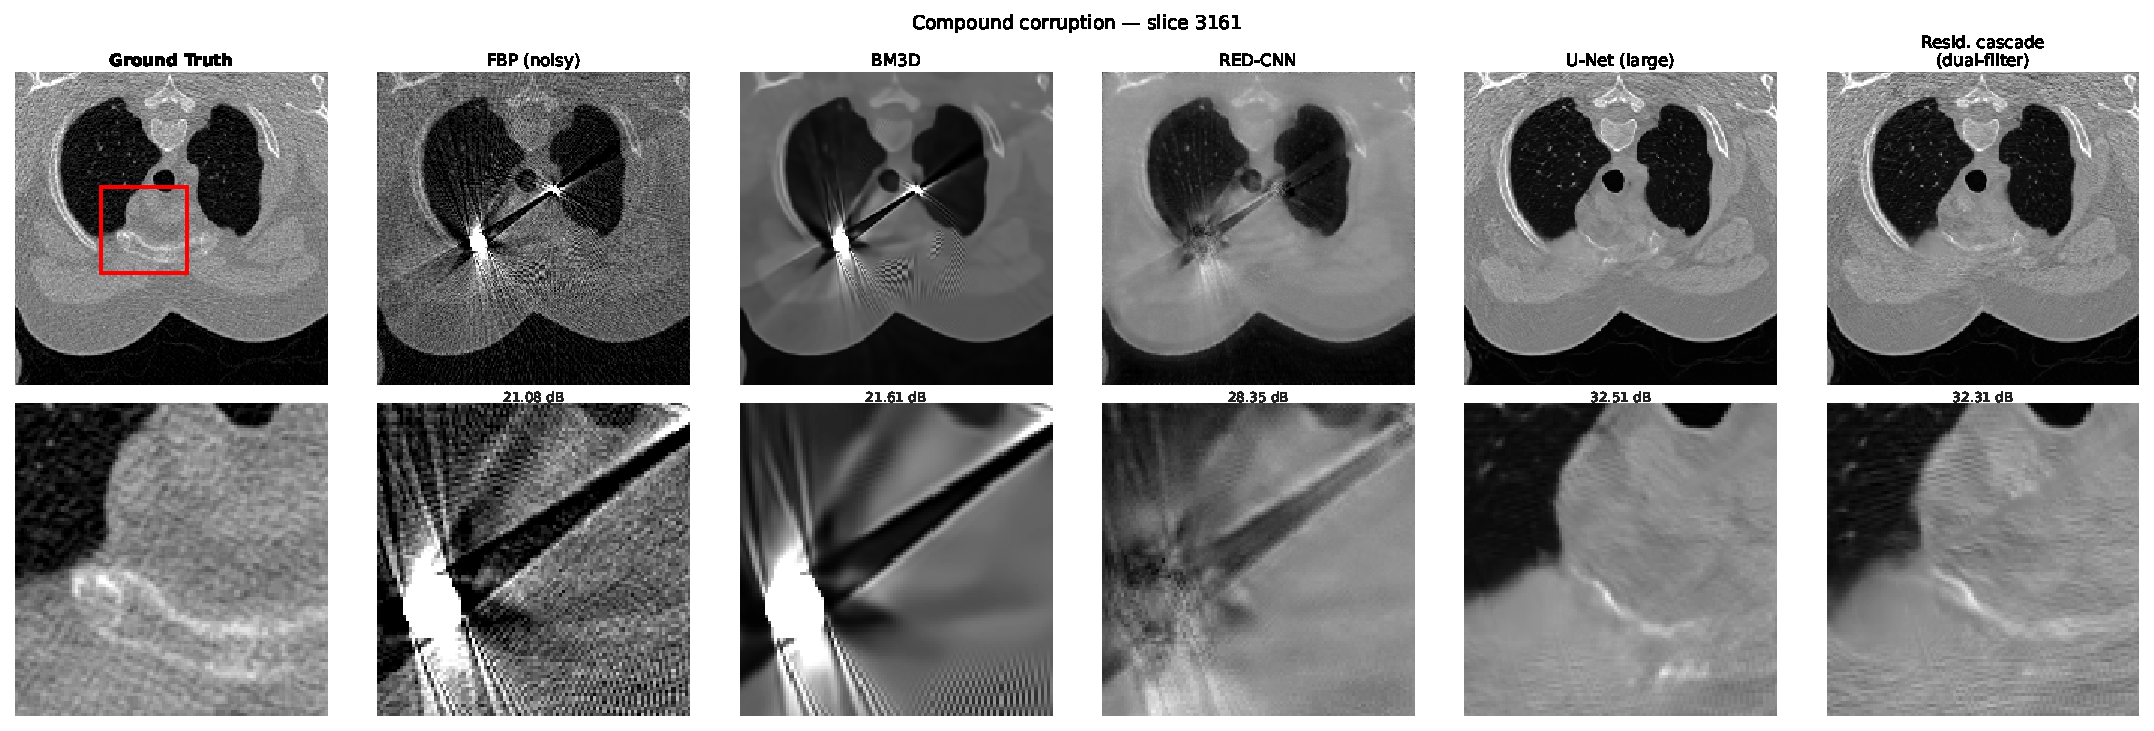
\includegraphics[width=\linewidth]{figures/results/fig_app_metal_slice3161.pdf}
    \caption[Slice~3161: metal artifact condition.]{%
        Slice~3161 with added metal implant artifacts (1--2 implants, scale
        0.10--0.30, photon-starvation clipping). Bright and dark saturation streaks
        are prominent in the FBP; the residual cascade with dual-filter input
        achieves the strongest streak suppression, visible in the zoomed crop.}
    \label{fig:app_qual_metal_3161}
\end{figure}

\begin{figure}[!htbp]
    \centering
    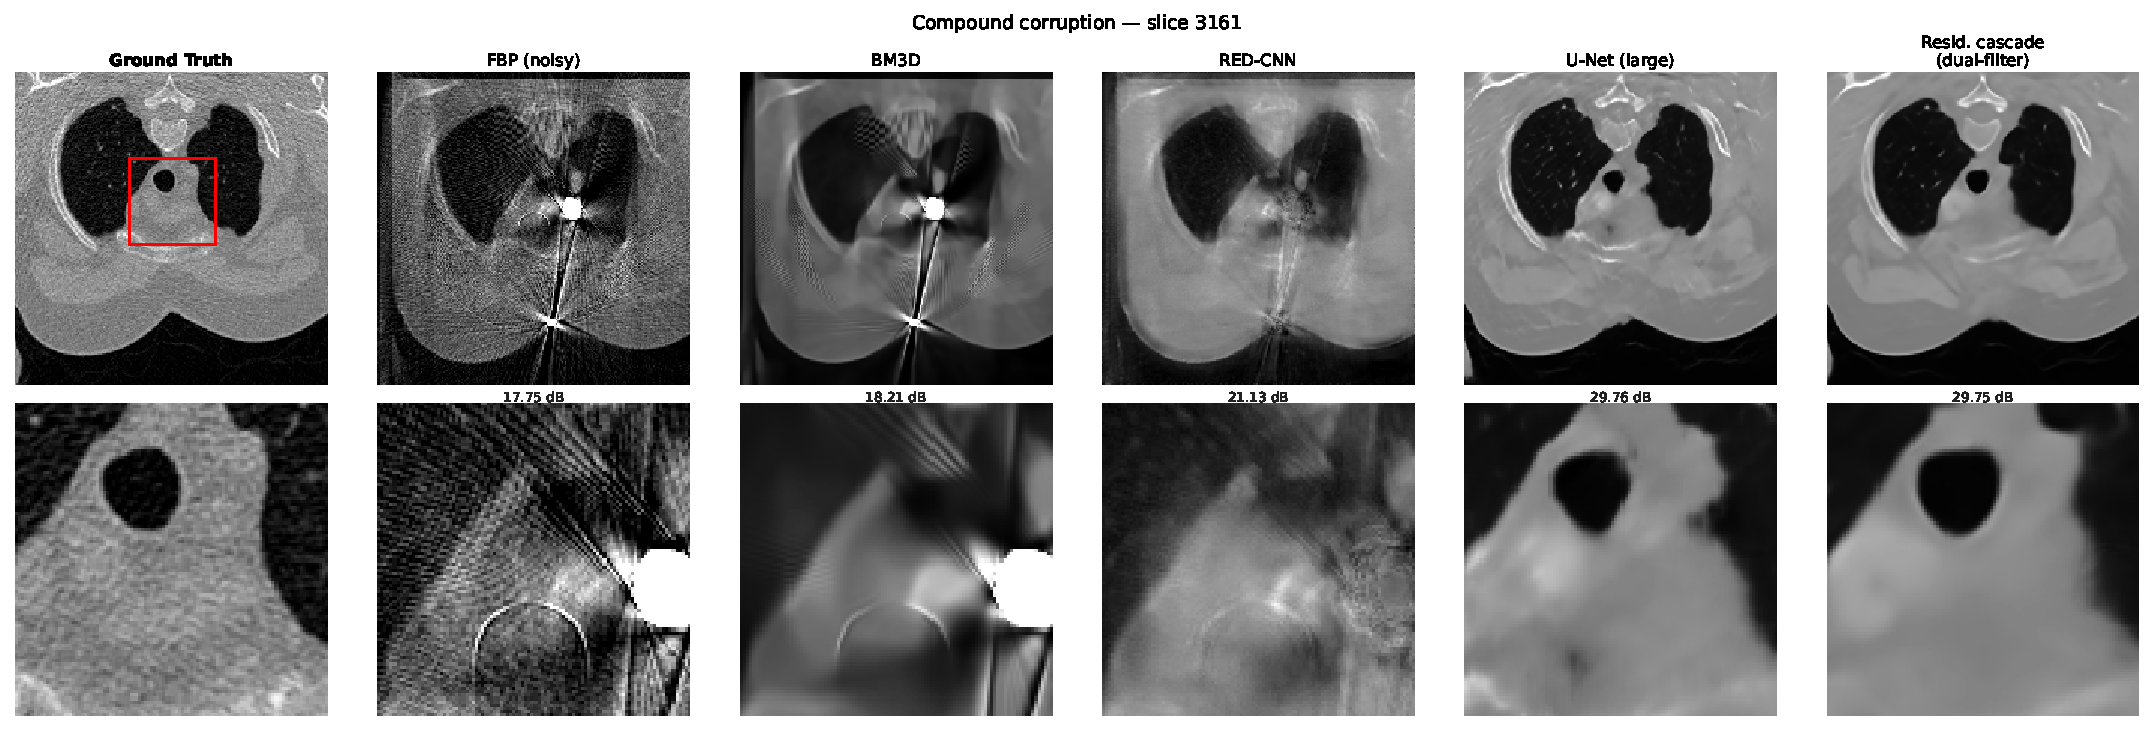
\includegraphics[width=\linewidth]{figures/results/fig_app_compound_slice3161.pdf}
    \caption[Slice~3161: compound corruption condition.]{%
        Slice~3161 under compound corruption (all three physical artifact types
        co-occurring simultaneously with Poisson noise). This is the hardest
        corruption regime evaluated in this thesis. The zoomed crop highlights
        the combined streak and ring pattern; the residual dual-filter cascade
        provides the most complete suppression.}
    \label{fig:app_qual_compound_3161}
\end{figure}

\section*{Slice 981}

\begin{figure}[!htbp]
    \centering
    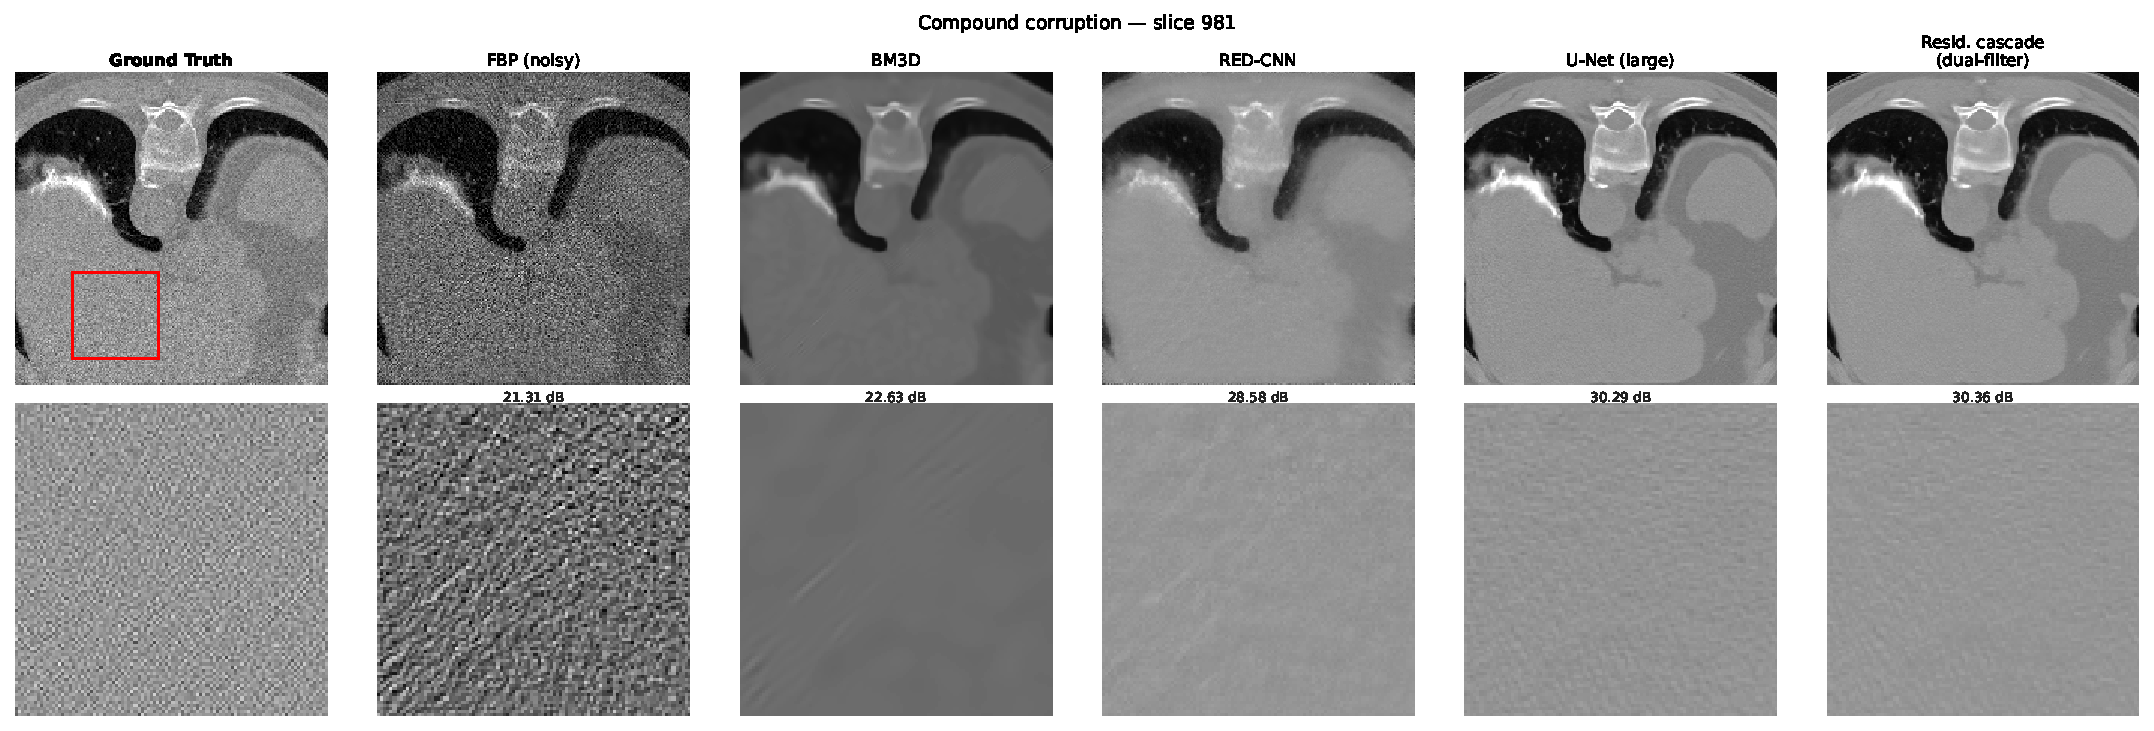
\includegraphics[width=\linewidth]{figures/results/fig_app_noise_only_slice0981.pdf}
    \caption[Slice~981: noise-only condition.]{%
        Slice~981, noise-only condition (low-dose Poisson noise only, no physical
        artifacts). All learned methods recover soft-tissue contrast suppressed by
        quantum noise; the residual dual-filter cascade and the large U-Net are
        visually indistinguishable at this corruption level, consistent with
        the per-artifact PSNR breakdown in \Cref{tab:exp_per_artifact}.}
    \label{fig:app_qual_noise_981}
\end{figure}

\begin{figure}[!htbp]
    \centering
    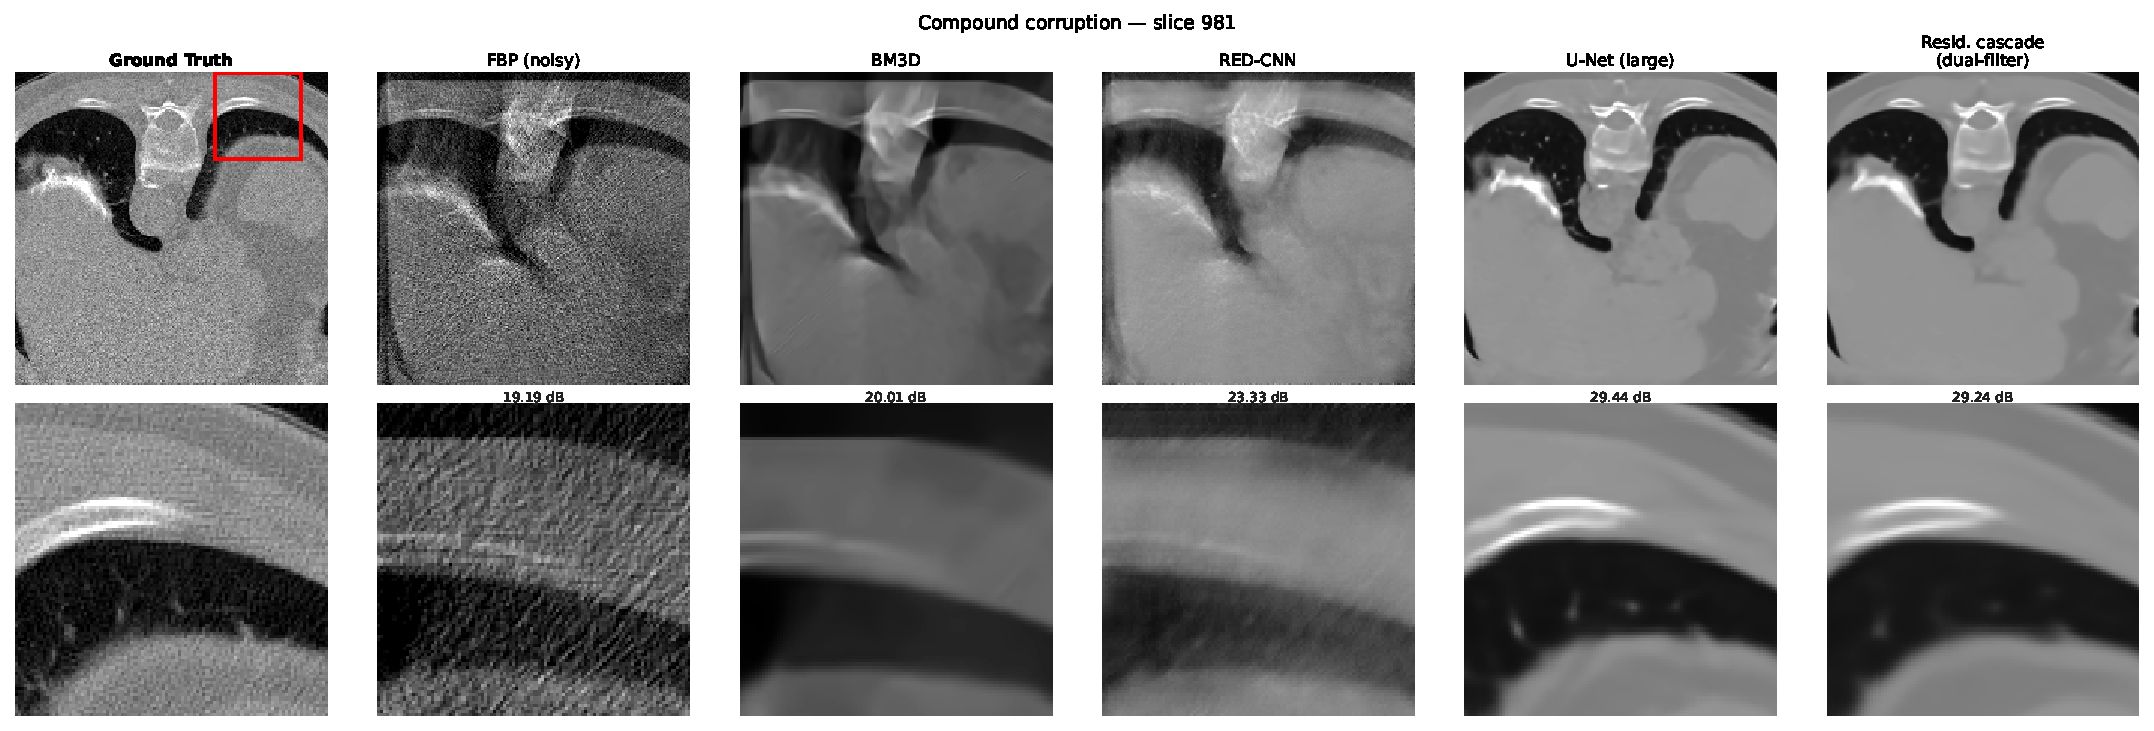
\includegraphics[width=\linewidth]{figures/results/fig_app_motion_slice0981.pdf}
    \caption[Slice~981: motion artifact condition.]{%
        Slice~981 with added respiratory motion artifacts (periodic sinogram shift,
        amplitude 10--20\,bins, 0.5--1.5 breathing cycles).
        The characteristic edge-blurring and double-contour effect is visible along
        lung-tissue boundaries in the corrupted FBP. Both U-Net variants suppress
        the blurring effectively; BM3D and RED-CNN partially reduce diffuse noise
        but leave the sinogram-domain inconsistency largely unresolved.}
    \label{fig:app_qual_motion_981}
\end{figure}

\begin{figure}[!htbp]
    \centering
    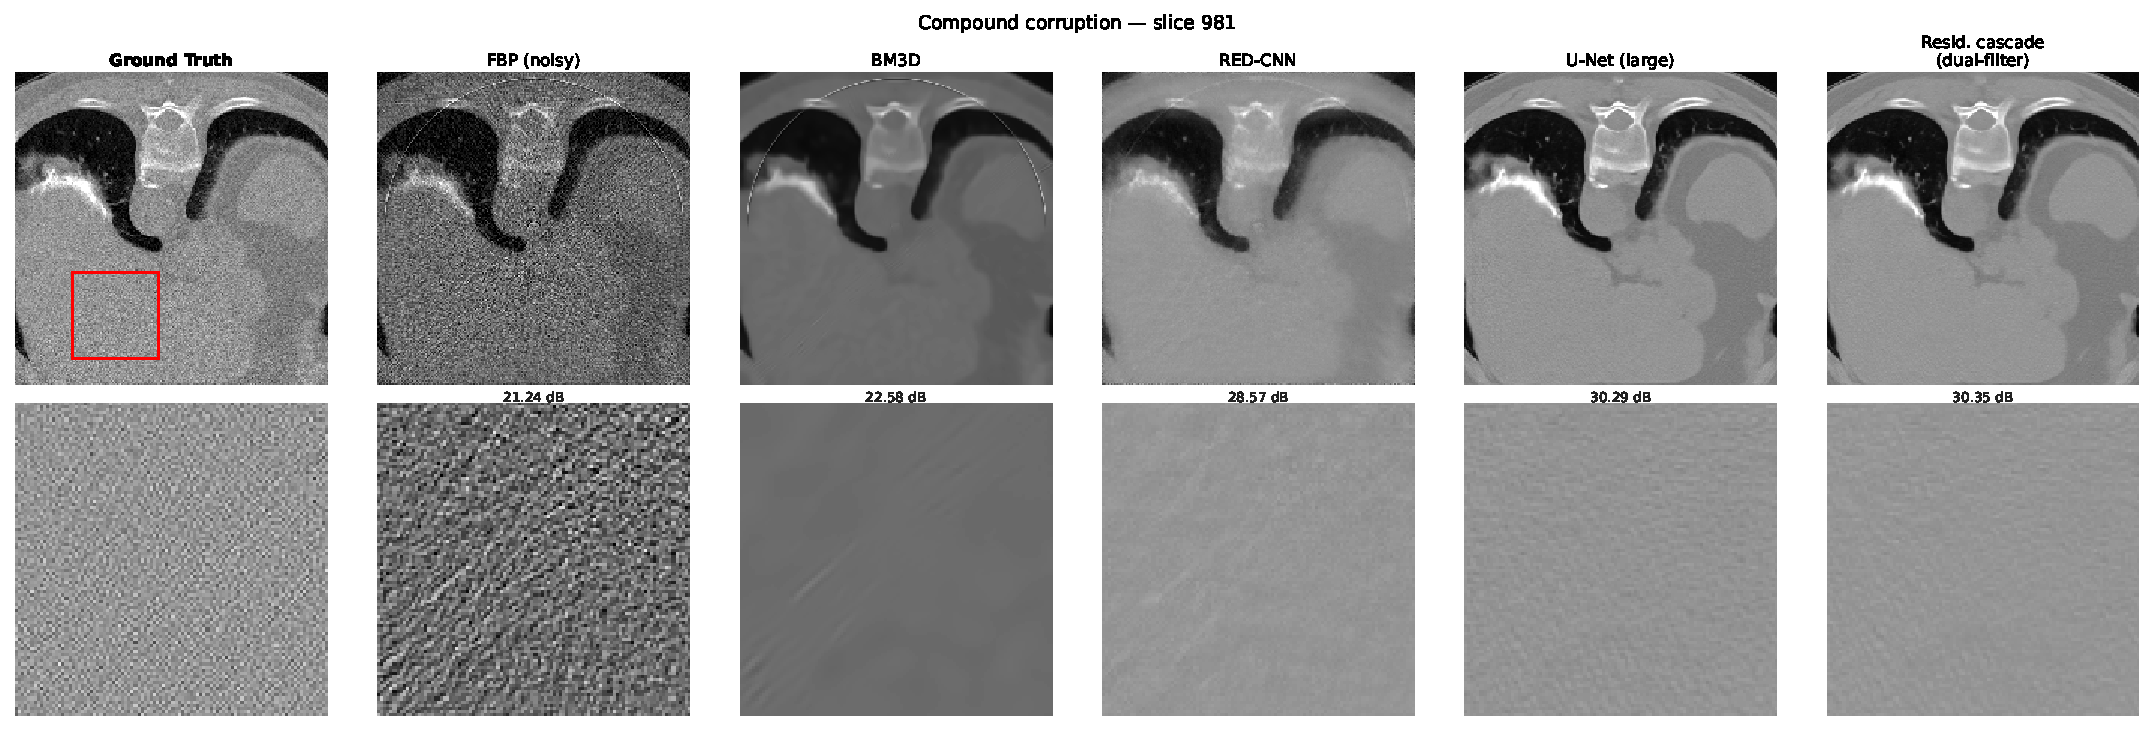
\includegraphics[width=\linewidth]{figures/results/fig_app_ring_slice0981.pdf}
    \caption[Slice~981: ring artifact condition.]{%
        Slice~981 with added detector ring artifacts (1--5 detector columns,
        gain error 5--50\,\%). Concentric rings of varying radii are visible
        in the FBP reconstruction, particularly near the image center. The
        learned models suppress ring patterns effectively while preserving
        surrounding soft-tissue contrast, consistent with the behavior observed
        in slice~3161 (\Cref{fig:app_qual_ring_3161}).}
    \label{fig:app_qual_ring_981}
\end{figure}

\begin{figure}[!htbp]
    \centering
    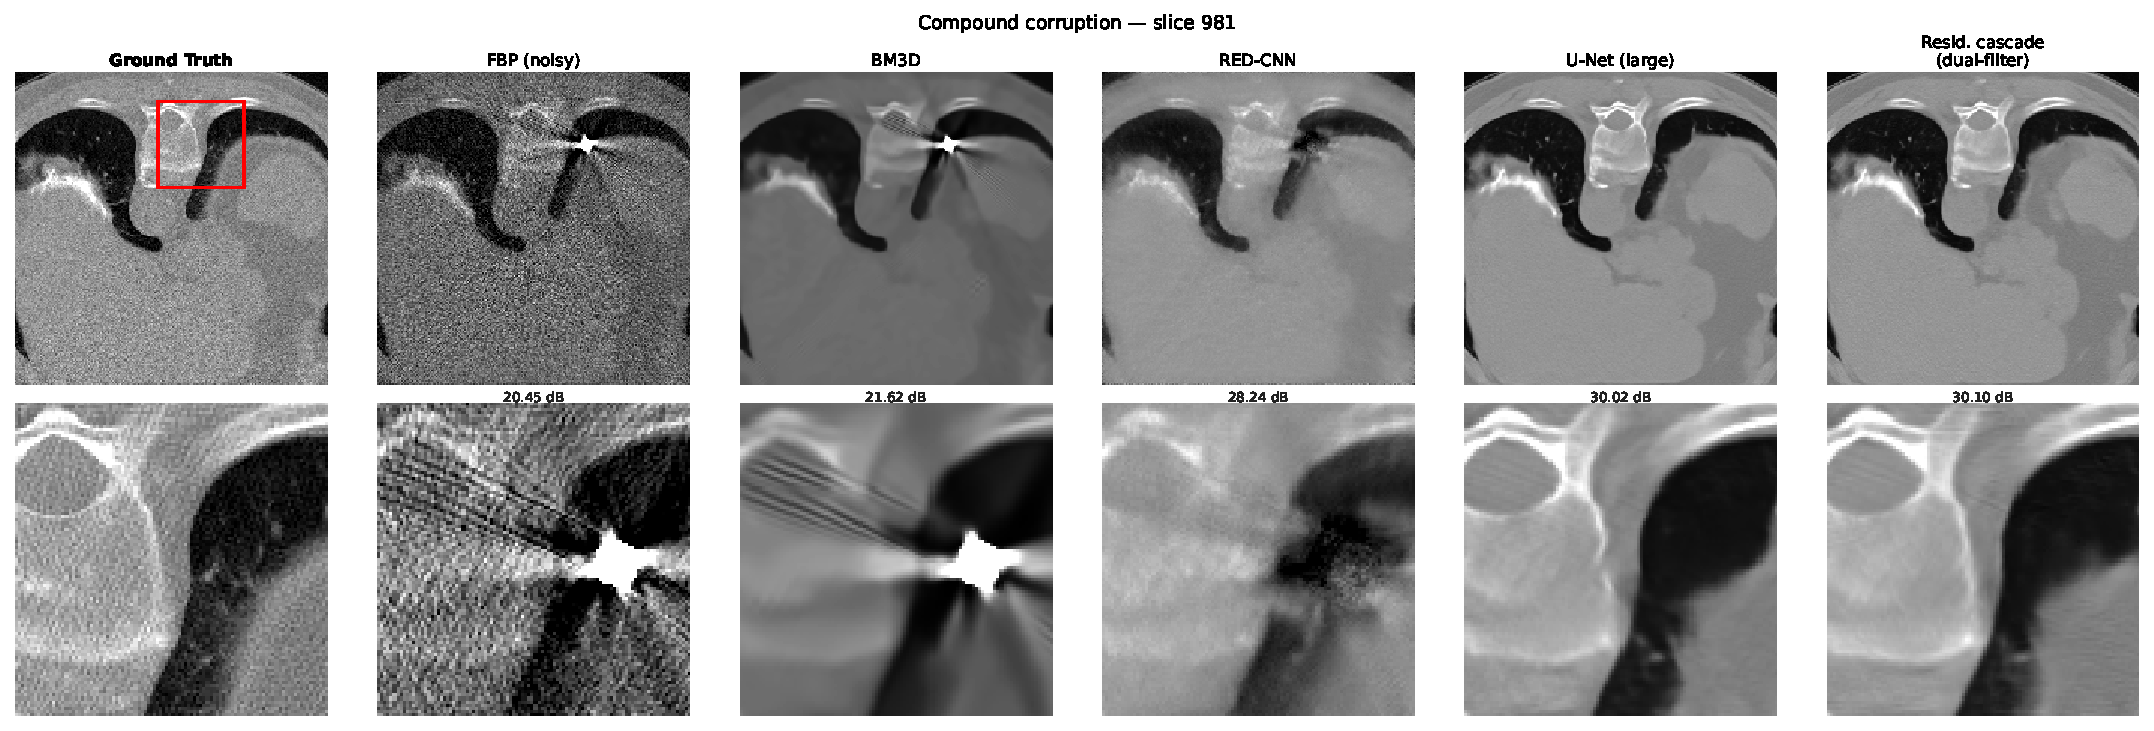
\includegraphics[width=\linewidth]{figures/results/fig_app_metal_slice0981.pdf}
    \caption[Slice~981: metal artifact condition.]{%
        Slice~981 with added metal implant artifacts (1--2 implants, effective
        attenuation scale 0.10--0.30, photon-starvation clipping active). Bright
        and dark saturation streaks are prominent in the FBP reconstruction. The
        residual dual-filter cascade achieves the strongest streak suppression
        among all methods, most clearly visible in the zoomed crop.
        RED-CNN reduces diffuse noise but leaves the highest-saturation streak
        regions largely unresolved.}
    \label{fig:app_qual_metal_981}
\end{figure}

\begin{figure}[!htbp]
    \centering
    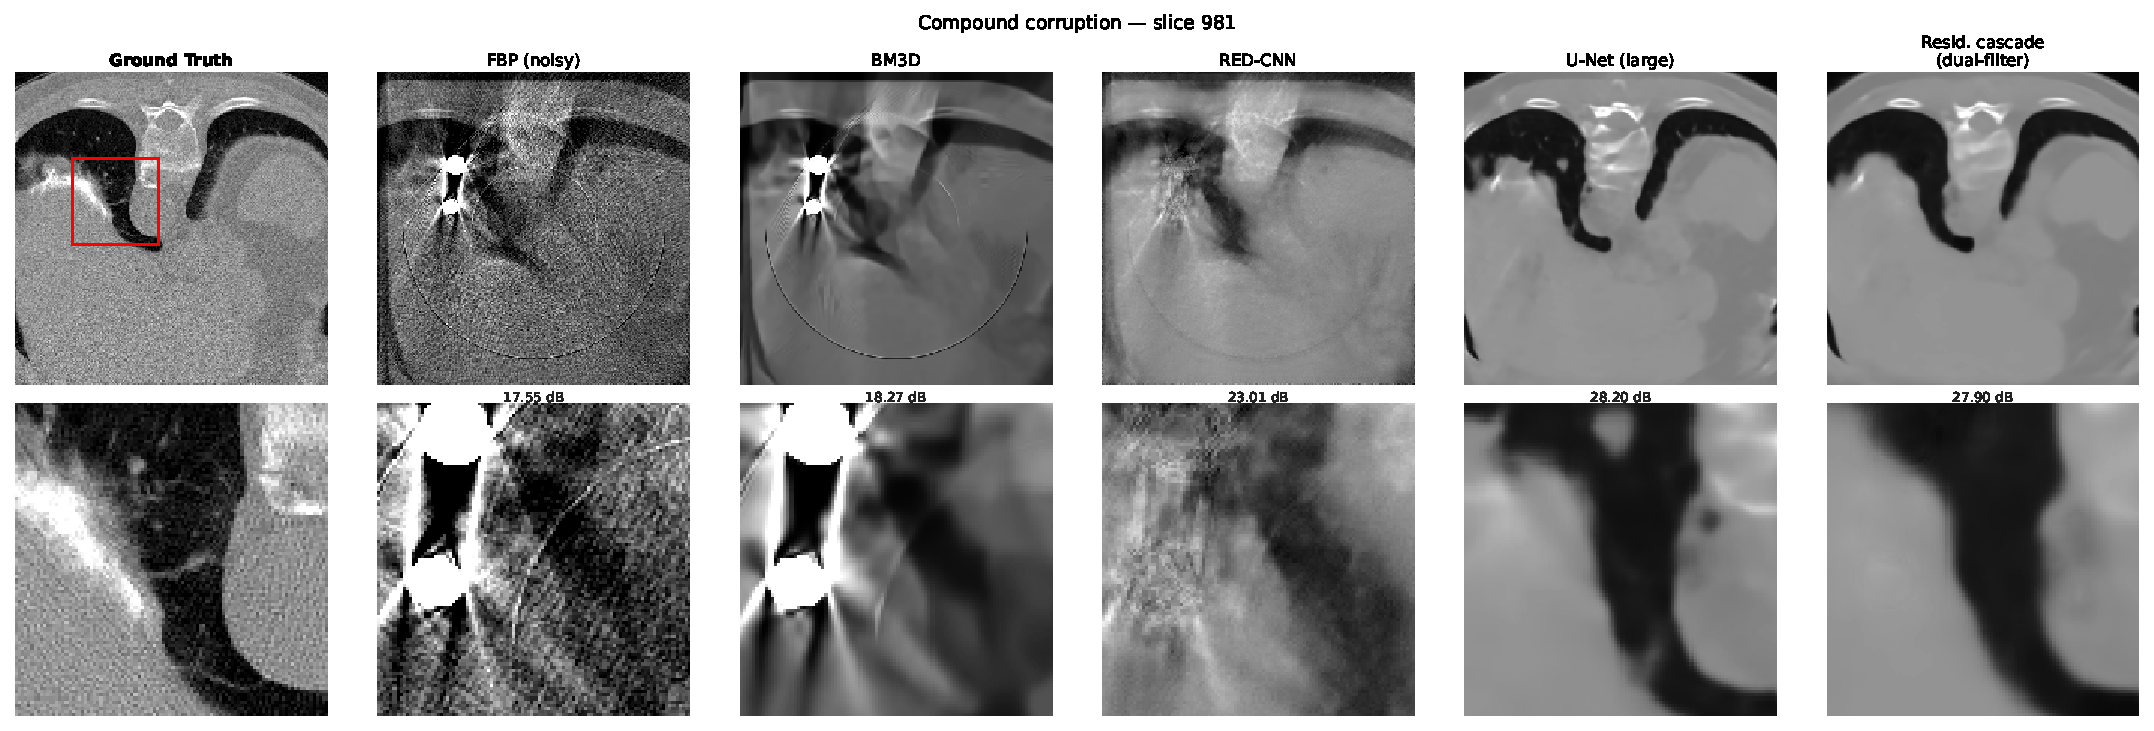
\includegraphics[width=\linewidth]{figures/results/fig_app_compound_slice0981.pdf}
    \caption[Slice~981: compound corruption condition.]{%
        Slice~981 under compound corruption (Poisson noise, motion, ring, and
        metal artifacts co-occurring simultaneously). This is the hardest
        corruption regime evaluated in this thesis. Both learned U-Net models
        substantially suppress the combined degradation, while BM3D and RED-CNN
        leave visible structured artifact residuals. The residual dual-filter
        cascade provides the most complete restoration in the zoomed crop, consistent
        with the quantitative results in \Cref{tab:exp_cascade}.}
    \label{fig:app_qual_compound_981}
\end{figure}

The per-artifact-count PSNR breakdown for all evaluated methods is reported in \Cref{tab:exp_per_artifact} in \Cref{chap:experiments}.


%%─────────────────────────────────────────────────────────
\chapter{Implementation Details and Hyperparameters}
\label{app:implementation}

\section*{Training hyperparameters}

\Cref{tab:app_hyperparams} provides the complete hyperparameter specification used for all models in this thesis. Hyperparameters shared across all cascade variants are listed in the upper block; model-specific settings are listed in the lower block.

\begin{table}[!htb]
    \centering
    \caption[Complete training hyperparameters.]{%
        Training hyperparameters shared across all model variants unless otherwise noted.}
    \label{tab:app_hyperparams}
    \setlength{\tabcolsep}{5pt}
    \small
    \begin{tabular}{@{}lll@{}}
        \toprule
        Hyperparameter & Value & Notes \\
        \midrule
        \multicolumn{3}{l}{\textit{Optimiser}} \\
        Algorithm       & AdamW & \\
        Learning rate   & $3\times10^{-4}$ & $1\times10^{-4}$ for RED-CNN \\
        $(\beta_1,\beta_2)$ & $(0.9,\,0.999)$ & \\
        Weight decay    & $10^{-2}$ & \\
        \midrule
        \multicolumn{3}{l}{\textit{Training schedule}} \\
        Epochs          & 150 (max) & early stopping, patience 15 \\
        Batch size      & 4 slices & \\
        Checkpoint selection & lowest validation loss & \\
        \midrule
        \multicolumn{3}{l}{\textit{Data}} \\
        Dataset         & LoDoPaB-CT~\cite{Leuschner2021} & \\
        Train / val / test split & 35\,820 / 3\,522 / 3\,553 & official split \\
        Corruption (train) & stochastic per epoch & fresh draw each epoch \\
        Corruption (val/test) & seeded: \texttt{seed\,+\,idx} & deterministic \\
        \midrule
        \multicolumn{3}{l}{\textit{Architecture (single-stage U-Net small)}} \\
        Encoder widths  & $[32,64,128,256]$ & \\
        Downsampling levels & 3 & $2\times2$ max-pool \\
        Upsampling      & bilinear + concat skip & \\
        Normalisation   & GroupNorm (8 groups) & \\
        Output activation & sigmoid & \\
        Parameters      & \num{1798113} & \\
        \midrule
        \multicolumn{3}{l}{\textit{Architecture (single-stage U-Net large)}} \\
        Encoder widths  & $[64,128,256,512]$ & \\
        Parameters      & \num{7184321} & \\
        \midrule
        \multicolumn{3}{l}{\textit{Loss weights}} \\
        Stage~1 loss    & $0.5\,\mathcal{L}_\mathrm{SSIM} + 0.5\,\mathcal{L}_1$ & \\
        Naive Stage~2 loss & $0.5\,\mathcal{L}_\mathrm{SSIM} + 0.5\,\mathcal{L}_1$ & \\
        Residual Stage~2 loss & $0.4\,\mathcal{L}_1(\hat{\mathbf{r}}) + 0.3\,\mathcal{L}_\mathrm{SSIM} + 0.3\,\mathcal{L}_\nabla$ & \\
        Cascade joint weight & $w_1=w_2=0.5$ & end-to-end only \\
        \midrule
        \multicolumn{3}{l}{\textit{Hardware}} \\
        GPU             & single NVIDIA GPU & \\
        Framework       & PyTorch & \\
        \bottomrule
    \end{tabular}
\end{table}

\section*{Code availability}

The full implementation, including the corruption pipeline, model definitions, training scripts, and evaluation notebooks, is available at \url{https://github.com/Mohammad-Shiblu/ct-restoration-cascade}. All seeded corruption draws and checkpoint files are included to allow exact reproduction of the reported results.


%%─────────────────────────────────────────────────────────
\chapter{Corruption Protocol Parameter Tables}
\label{app:protocol_params}

The corruption protocol is fully specified in \Cref{sec:meth_compound}. For convenience, \Cref{tab:app_motion_params,tab:app_ring_params,tab:app_metal_params,tab:app_compound_probs} reproduce the parameter tables from \Cref{chap:methodology} and add the compound activation statistics in one place.

\begin{table}[!htb]
    \centering
    \caption[Motion artifact parameters (reproduced from \Cref{tab:meth_motion_params}).]{%
        Sampling ranges for the motion artifact model. See \Cref{sec:meth_motion} for derivation.}
    \label{tab:app_motion_params}
    \begin{tabular}{llll}
        \toprule
        Parameter & Symbol & Range & Physical interpretation \\
        \midrule
        Peak detector shift     & $A$            & $[10,20]$ bins & $\approx7$--$14\,\text{mm}$ motion \\
        Breathing cycles / scan & $f$            & $[0.5,1.5]$    & quasi-periodic respiration \\
        Initial phase           & $\varphi$      & $[0,2\pi)$     & random scan-start phase \\
        Activation probability  & $p_\text{mot}$ & $0.5$          & \\
        \bottomrule
    \end{tabular}
\end{table}

\begin{table}[!htb]
    \centering
    \caption[Ring artifact parameters (reproduced from \Cref{tab:meth_ring_params}).]{%
        Sampling ranges for the ring artifact model. See \Cref{sec:meth_ring} for derivation.}
    \label{tab:app_ring_params}
    \begin{tabular}{llll}
        \toprule
        Parameter & Symbol & Range & Physical interpretation \\
        \midrule
        Affected columns        & $|\mathcal{C}|$ & $\{1,\dots,5\}$  & sparse detector faults \\
        Detector gain           & $g_c$           & $[0.5,0.95]$     & $5$--$50\,\%$ calibration error \\
        Implied offset          & $|c_c|$         & $[6.3\times10^{-4},8.5\times10^{-3}]$ & $\mu_{\max}$-normalized \\
        Activation probability  & $p_\text{ring}$ & $0.5$            & \\
        \bottomrule
    \end{tabular}
\end{table}

\begin{table}[!htb]
    \centering
    \caption[Metal artifact parameters (reproduced from \Cref{tab:meth_metal_params}).]{%
        Sampling ranges for the metal artifact model. See \Cref{sec:meth_metal} for derivation.}
    \label{tab:app_metal_params}
    \setlength{\tabcolsep}{4pt}
    \small
    \begin{tabular}{@{}llll@{}}
        \toprule
        Parameter & Symbol & Range & Physical interpretation \\
        \midrule
        Number of implants      & $N_\mathrm{impl}$  & $\{1,2\}$           & \\
        Mask radius             & $r_\mathrm{impl}$  & $[3,12]\,\text{px}$ & $\approx2$--$9\,\text{mm}$ \\
        Metal strength          & $\alpha$           & $[0.10,0.30]$       & effective attenuation \\
        Radial position         & $r/H$              & $[0.05,0.35]$       & inside FOV \\
        Activation probability  & $p_\mathrm{metal}$ & $0.3$               & \\
        \bottomrule
    \end{tabular}
\end{table}

\begin{table}[!htb]
    \centering
    \caption[Expected compound artifact distribution.]{%
        Expected fraction of training samples carrying each artifact count, derived analytically
        from the independent Bernoulli gates with
        $(p_\mathrm{mot}, p_\mathrm{ring}, p_\mathrm{metal}) = (0.5, 0.5, 0.3)$.}
    \label{tab:app_compound_probs}
    \begin{tabular}{lc}
        \toprule
        Number of additional physical artifacts & Expected fraction \\
        \midrule
        0 (noise only)  & $17.5\,\%$ \\
        1               & $42.5\,\%$ \\
        2               & $32.5\,\%$ \\
        3               & $7.5\,\%$  \\
        \bottomrule
    \end{tabular}
\end{table}
